\begin{enumerate}[label=\thesection.\arabic*.,ref=\thesection.\theenumi]
\numberwithin{equation}{enumi}

\item  Find the cross-over frequency of the  given transfer function :
\begin{align}
\label{eq:es17btech11019_system}
G(s) &= \cfrac{100}{(s+1)^3}
\end{align}
\\
\solution The phase crossover is a frequency at which phase angle first reaches -180 degree or at which frequency the imaginary part of denominator of transfer function is equal to zero.The corresponding frequency is the phase crossover frequency.


\begin{align}
G(j\omega)=\cfrac{100}{(j\omega+1)^3}
\end{align}
\begin{align}
 &= \cfrac{100}{(1-3\omega^2)+j(3\omega-\omega^3)}
\end{align}
     
Now equating the imaginary part to zero
\begin{align}
(3\omega-\omega^3)=0
\end{align}  
\begin{align}
\implies \omega = \sqrt{3}
\end{align}

As phase should be greater than zero for stability.

\item Verify using the Nyquist plot.
\\
\solution Use the following matlab code to generate the Nyquist plot in Fig.  \ref{fig:es17btech11019}
\begin{lstlisting}
codes/es17btech11019.m
\end{lstlisting}
%
\begin{figure}[!h]
\centering
  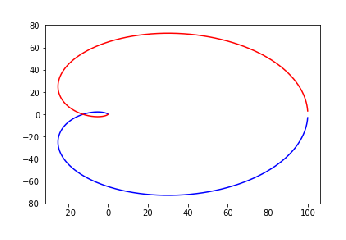
\includegraphics[width=\columnwidth]{./figs/es17btech11019.eps}
  \caption{}
  \label{fig:es17btech11019}
\end{figure}


Conclusion: As we can see from the figure, the point where nyquist plot passes is
\begin{align}
{\omega=\sqrt{3}}
\end{align}
that is 1.73 and as it is positive so the system is stable.


\end{enumerate}
